\documentclass[a4paper, 11pt]{article}

\usepackage[utf8]{inputenc}
\usepackage[T1]{fontenc}
\usepackage[super]{natbib}
\usepackage[french]{babel}
\usepackage{helvet}
\usepackage[top=35mm, bottom=35mm, left=25mm, right=25mm]{geometry}
\usepackage{geometry}
\usepackage{graphicx}
\usepackage{multirow}  
\usepackage{subfigure}
\usepackage{verbatim}
\usepackage{url}
\usepackage{algorithm2e, algorithmic} 
\usepackage{amsmath,amsfonts,amssymb}
\usepackage{lmodern}
\usepackage{microtype}
\usepackage{xcolor}
\usepackage{textcomp}
\usepackage{minted}
\usepackage{framed}
\usepackage{tcolorbox}
\usepackage{wrapfig}
\usepackage{etoolbox}
\usepackage{multicol}
\usepackage{caption}
\BeforeBeginEnvironment{minted}{\begin{tcolorbox}[left=8mm]\begin{center}}
\AfterEndEnvironment{minted}{\end{center}\end{tcolorbox}}%
\usepackage{hyperref}
\hypersetup{
pdfpagemode={},
pdfstartview={XYZ 3000 3000 0.75}
pdfstartview={XYZ left top zoom}
}
\hypersetup{
pdftitle={M1 ISICG - Introduction au Traitement Numérique des Images},
pdfsubject={Rapport de projet},
pdfauthor={Rouijel Mehdi},
pdfkeywords = {M1, ISICG, Traitement, Images, Numérique, Université de Limoges, Faculté des Sciences et Techniques}
}
\setcounter{secnumdepth}{3}

\usepackage{fancyhdr}
%\pagestyle{fancy}
% \lhead{}
% \rhead{}
\fancypagestyle{plain}{%
\fancyhf{} % clear all header and footer fields
\fancyfoot[C]{\fontfamily{\familydefault}\fontsize{10pt}{14pt}\selectfont page \thepage} % except the center
\renewcommand{\headrulewidth}{1pt}
\renewcommand{\footrulewidth}{1pt}}
\pagestyle{plain}


\renewcommand{\familydefault}{phv}
%\renewcommand{\familydefault}{\sfdefault}

\definecolor{unilim_blue}{HTML}{103147}
\definecolor{unilim_red}{HTML}{9e3232}

\hypersetup{
    colorlinks,
    citecolor=unilim_red,
    filecolor=unilim_red,
    linkcolor=unilim_red,
    urlcolor=unilim_red,
}

\renewcommand{\thesection}{\color{unilim_red}\textsc\Roman{section}}
\renewcommand{\thesubsection}{\color{unilim_red}\textsc\thesection-\Roman{subsection}}


\begin{document}

%
%  -------
% | TITLE |
%  -------
%

\begin{titlepage}
\setlength{\headheight}{0cm}
\setlength{\headsep}{0cm}
{
  \noindent
  \begin{tabular}[t]{@{}l}
    \small\textsc{Université de Limoges}\\
    \small{Faculté des Sciences et Techniques}
  \end{tabular}
  \hfill
  \begin{tabular}[t]{l@{}}
    \small{Année Universitaire 2016 - 2017}
  \end{tabular}
  
  \vspace{-5.5mm}
  \begin{figure}[!h]
	\hspace*{-7.5mm}
\includegraphics[height=20mm]{img/unilim-fst.jpg}
  \end{figure}
      
  \vspace{20mm}
  \begin{center}
    
    \large\underline{Master \textsc{Informatique} ISICG, semestre 2}\\
    \Large\textsc{traitement numérique des images}
    
    \vspace{15mm}
  
    \begin{tcolorbox}[colback=unilim_blue, colframe=unilim_blue, boxrule=0.5pt, arc=4pt,
                      left=6pt, right=6pt, top=6pt, bottom=6pt, boxsep=0pt]
      \begin{minipage}[h]{\linewidth}
        \begin{center}
        { \color{white}
          \vspace*{5mm}
          \huge\textsc{Détection de Cibles de Fléchettes}\\
          \vspace*{5mm}
          \Large\textbf{\underline{Rapport de projet}}
          \vspace*{5mm}
        }
        \end{center}
      \end{minipage}
    \end{tcolorbox}
    
    \vspace{2mm}
    
    \large{version du \today}
    \vspace{25mm}\\
    Auteur\\~\\
    {
    \large
    \bsc{Rouijel} Mehdi
    }
    
  \end{center}
  
  \vfill
  \begin{flushleft}
	Responsable  : M. \bsc{Crespin} Benoît\\
  \end{flushleft}
}
\end{titlepage}

\clearpage


%
%  ---------
% | CONTENT |
%  ---------
%

\section*{\color{unilim_red}\textsc{Introduction}}
\par
L'objectif de ce projet est de mettre en pratique les notions vues en cours, en particulier la transformée de Hough, en créant une application capable de détecter une cible de fléchettes dans une image. Au-delà de la simple détection de la cible, le programme devrait pouvoir reconnaître ses différentes zones ainsi que les numéros autour; si des fléchettes sont présentes dans l'images, elles devraient être détectées aussi, pour éventuellement être capable de déterminer le score.

\bigskip
\bigskip

\begin{multicols}{2}

\section{Utilisation de l'application}
\par
Une fois l'application lancée depuis Eclipse, une image par défaut est chargée. Pour utiliser une autre image, il suffit de naviguer vers \og File > Open... \fg{} pour sélectionner une nouvelle image. Il est aussi possible de sauvegarder l'image qui est vue dans la partie droite de la fenêtre, après avoir exécuté une opération, en utilisant \og File > Save... \fg{}. La copie (\og Edit > Copy \fg{}) n'est pas implémentée.
\par
Chaque bouton du panneau de contrôle est indépendant. Par exemple, il est possible de n'appliquer que le flou, mais c'est l'image originale, et non le résultat de celui-ci, qui sera utilisée si la détection des contours est appliquée ensuite.
\par
Différents paramètres peuvent être changés, en ouvrant la barre d'options du panneau de contrôle, pour la détection de contours, la détection de lignes et la détection d'ellipses ; elles sont expliquées dans la suite de ce rapport. Modifier ces paramètres aura un effet important sur le résultat final.

\section{Détection des contours}
\par
La détection des contours se fait par une application du filtre de Sobel qu'il est possible d'améliorer grâce aux différentes options disponibles dans le panneau de contrôle. Sélectionner l'ensemble des options rapproche le traitement d'un filtre de Canny \cite{wiki_canny}, avec dans l'ordre :
\begin{enumerate}
\item Réduction du bruit par un filtre de Gauss
\item Seuillage
\item Analyse de région (\og blob analysis \fg{})
\item Amincissement
\end{enumerate}
%\begin{wrapfigure}{r}{0.35\textwidth}
\begin{center}
%\vspace{-1mm}
\centering
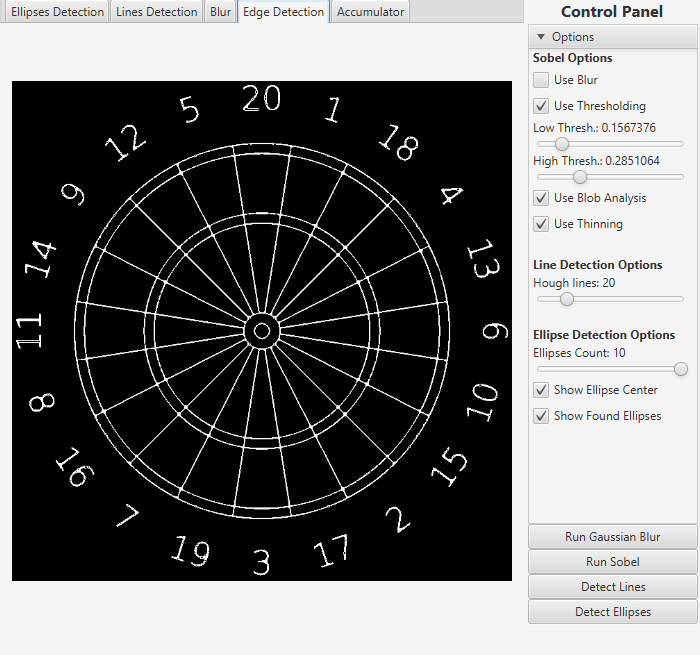
\includegraphics[width=0.9\linewidth]{img/front_edges_00.png}
\vspace{-2mm}
\captionof{figure}{Contours trouvés}
\label{fig:frontEdges00}
\end{center}
%\end{wrapfigure}
\par
Il est à noter que deux seuils peuvent être modifiés. Le seuil haut concerne l'étape de seuillage et détermine la valeur frontière pour séparer les pixels affichés des pixels de fond. Le seuil bas est utilisé par l'analyse locale ; celle-ci ne pourra d'ailleurs fonctionner que si le seuillage est aussi sélectionné.
\par
Le fonctionnement de l'analyse locale est simple : lors de l'étape de seuillage, les pixels au-dessus du seuil haut sont marqués comme \og forts \fg{} et les pixels entre les deux seuils sont marqués comme \og faibles \fg{}. Par la suite, un pixel faible ne sera gardé que s'il est connecté à un pixel fort. En fonction de l'image, nous pouvons constater une amélioration du résultat.

\section{Détection des lignes}
Le programme utilise la transformée de Hough pour détecter les lignes.
\begin{center}
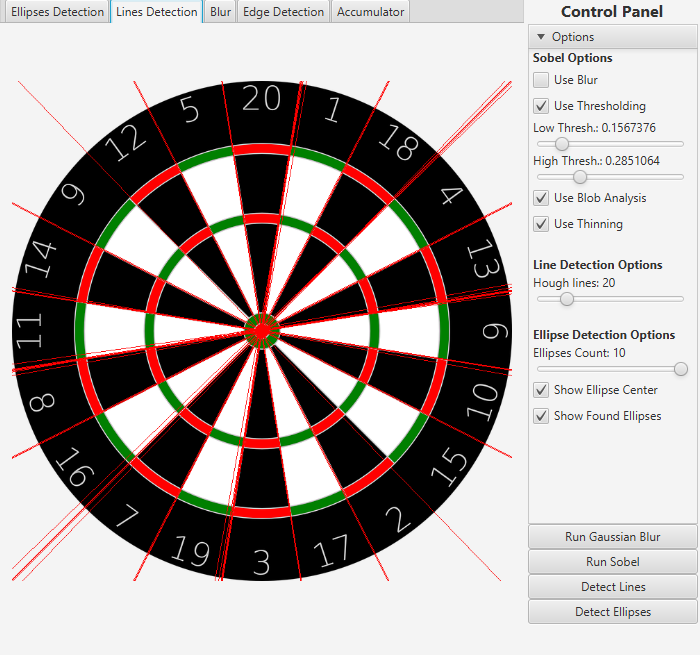
\includegraphics[width=0.9\linewidth]{img/front_lines_00.png}
\vspace{-2mm}
\captionof{figure}{Lignes trouvées}
\label{subfig:frontLines00}
\end{center}

\par
Dans l'image obtenue par la détection de contours, on regarde les $i$ pixels blancs. Chacun de ces pixels appartient aux droites à une distance $\rho_{i}$ de l'origine, et orientées à un angle $\theta_{i}$ sur l'intervalle $[0..2\pi]$; dans une matrice de taille $\rho_{max}\times\theta_{max}$, nous incrémentons alors la case correspondante. Plus il y a de pixels le long d'une droite, plus la valeur de la case $(\rho,\theta)$ associée sera élevée, et donc plus il est probable que nous ayons détecté une ligne.
\par
Il ne nous reste plus qu'à récupérer les $n$ valeurs les plus élevées pour tracer les $n$ droites détectées en repassant du système polaire au système cartésien grâce aux équivalences $x = \rho \cdot \cos\theta$ et $y = \rho \cdot \sin\theta$.

\section{Détection des ellipses}
\par
Dans le cas de cibles de fléchettes, la majorité des lignes trouvées devraient être les délimitations des sections qui convergent vers le centre. Cependant, la détection de lignes n'est jamais exacte, nous aurons donc plusieurs points d'intersection proche du \og vrai \fg{} centre.
\par
Pour déterminer le centre qui sera utilisé, nous regardons les lignes deux à deux et mémorisons leur intersection. Une procédure en \og force brute \fg{} détermine ensuite les deux intersections les plus proches, puis le centre choisi sera la moyenne de ces deux intersections.

\end{multicols}

\begin{figure}[!h]
\centering
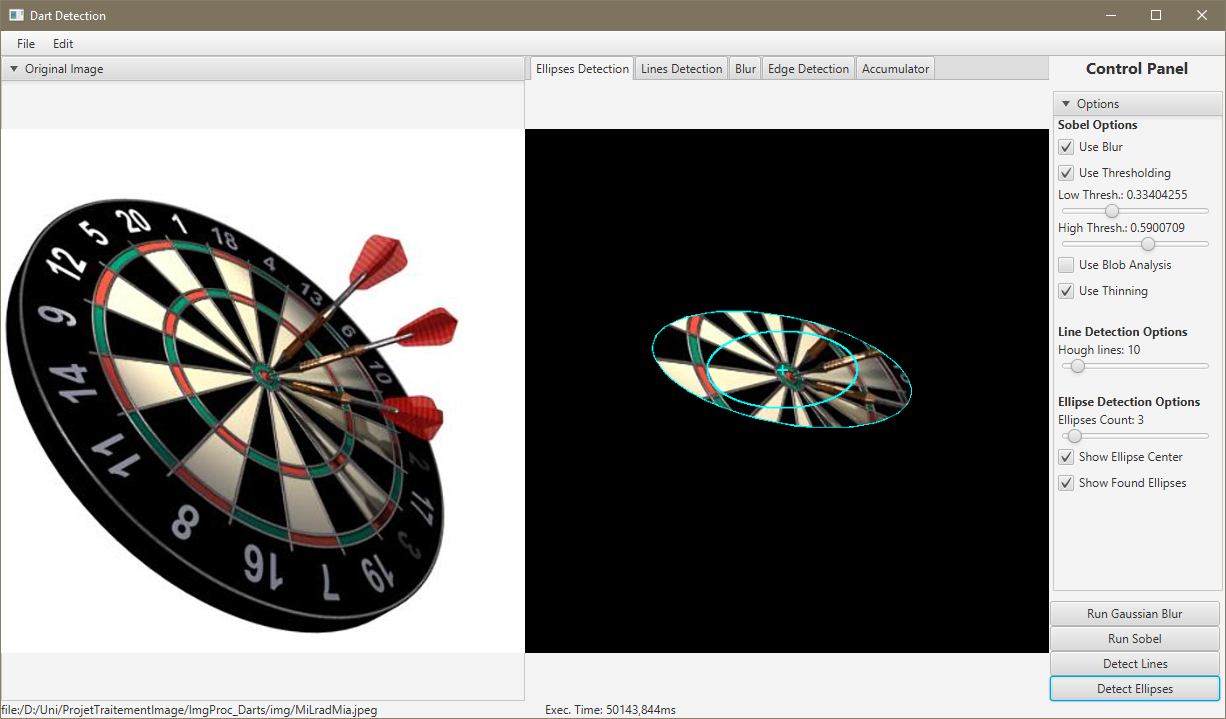
\includegraphics[width=0.85\linewidth]{img/rotated_result_00.png}
\vspace{-2mm}
\caption{Résultat non convaincant}
\label{fig:rotatedResult00}
\end{figure}

\begin{multicols}{2}

\par
\`A partir de ce centre, les combinaisons possibles de rayons et d'angles de rotation sont regardées et comparées avec l'image issue de la détection de contours. C'est, là aussi, un procédé en \og force brut \fg{} qui est relativement lent pour un résultat très discutable, comme le montre la figure \ref{fig:rotatedResult00}.
\par
Le résultat obtenu peut néanmoins être amélioré en jouant avec les paramètres, et est acceptable dans le cas d'une cible vue de face et suffisamment éclairée (c.f. Figure \ref{fig:frontResult00}).

\section{Travail non réalisé}
\par
Par manque de temps, la détection des nombres, des sections de la cible et des fléchettes prévues pour ce projet ne sont pas implémentées.
\par
La détection des sections nécessiterait une détection des ellipses plus précise qui, combinée avec la détection de lignes, pourrait permettre un étiquetage des zones trouvées.
\par
La détection des nombres et des fléchettes sont plus complexes et demanderaient plus de réflexion.

\end{multicols}

\begin{figure}[!h]
\centering
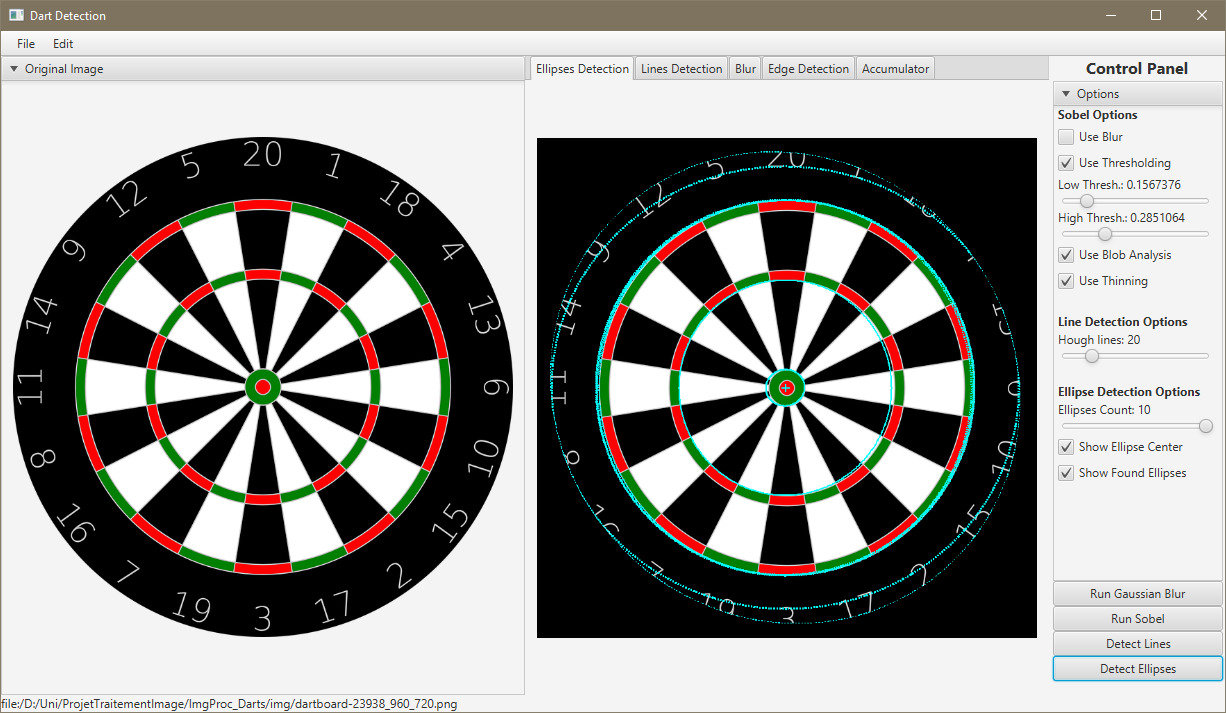
\includegraphics[width=0.85\linewidth]{img/front_result_00.png}
\vspace{-2mm}
\caption{Résultat de la détection d'ellipses avec \ref{fig:frontEdges00} et \ref{subfig:frontLines00}}
\label{fig:frontResult00}
\end{figure}

\bigskip
\bigskip

\section*{\color{unilim_red}\textsc{Conclusion}}
\par
Les résultats obtenus ne sont pas satisfaisants. Au-delà des fonctionnalités manquantes, il serait possible d'améliorer le code existant à plusieurs niveaux.
\par
Sur le plan de la conception globale de l'application, nous pourrions procéder à quelques ajustement; elle suit assez librement le patron de conception MVC et son implémentation pourrait être plus stricte.
\par
Ensuite, les procédures en \og force brute \fg{} évoquées plus haut dans le rapport pourraient être remplacées. Pour la recherche des points les plus proches, notamment, il existe plusieurs algorithmes qui permettraient de réduire le temps d'exécution, surtout pour un nombre de lignes élevé.
\par
Enfin, avec une détection d'ellipses plus précise, il serait possible de déterminer si l'objet détecté est bien une cible, par exemple grâce au nombre d'ellipses concentriques. En l'état, l'application ne serait pas capable de faire la différence entre une cible et une roue de vélo.

\clearpage

%
%  --------------
% | BIBLIOGRAPHY |
%  --------------
%
  
\nocite{*}
\bibliographystyle{unsrt}
\bibliography{M1_TraitementImages_ROUIJEL}


\end{document}
